\documentclass[12pt,a4paper]{article}

\usepackage[margin=1in]{geometry}
\usepackage[pdftex]{hyperref}
\usepackage{amsmath,amsthm,amssymb,graphicx,mathtools,tikz,hyperref,enumerate}
\usepackage{mdframed,cleveref,cancel,stackengine,pgfplots,subcaption,pgf}
%\usepackage[spanish]{babel}

\newmdenv[leftline=false,topline=false]{topright}
\let\proof\relax
\usepackage[utf8]{inputenc}
\usetikzlibrary{positioning}
\newcommand{\n}{\mathbb{N}}
\newcommand{\z}{\mathbb{Z}}
\newcommand{\q}{\mathbb{Q}}
\newcommand{\cx}{\mathbb{C}}
\newcommand{\real}{\mathbb{R}}
\newcommand{\E}{\mathbb{E}}
\newcommand{\F}{\mathbb{F}}
\newcommand{\D}{\mathcal{D}}
\newcommand{\bb}[1]{\mathbb{#1}}
\let\k\relax
\newcommand{\k}{\mathbf{k}}
\newcommand{\ita}[1]{\textit{#1}}
\newcommand{\inv}[1]{#1^{-1}}
\newcommand\setb[1]{\left\{#1\right\}}
\newcommand{\vbrack}[1]{\langle #1\rangle}
\newcommand{\determinant}[1]{\begin{vmatrix}#1\end{vmatrix}}
\newcommand{\abs}[1]{\left\vert #1 \right\vert}
\newcommand{\Po}{\mathbb{P}}

\newcommand{\dualpar}[1]{\left(#1\right)^\ast}
\newcommand{\dual}[1]{#1^\ast}

\DeclareMathOperator{\join}{\vee}
\DeclareMathOperator{\Id}{Id}
\DeclareMathOperator{\rg}{rg}
\DeclareMathOperator{\car}{car}

\newcommand{\myref}[1]{\hyperref[item:a#1]{\uppercase{a#1}}}


\hypersetup{
	colorlinks,
	linkcolor=blue
}

\usetikzlibrary{arrows}

\newtheoremstyle{break}% name
{}%         Space above, empty = `usual value'
{}%         Space below
{}% Body font
{}%         Indent amount (empty = no indent, \parindent = para indent)
{\bfseries}% Thm head font
{}%        Punctuation after thm head
{\newline}% Space after thm head: \newline = linebreak
{#1 #2 \normalfont \textit{#3}}%         Thm head spec


\theoremstyle{break}
\newtheorem{ej}{Ejercicio}
\newtheorem{defi}{Definición}
\let\proof\relax
\newtheorem*{proof}{Solución}

%\pgfplotsset{compat=1.5}

\begin{document}
\date{}

\title{\textbf{Álgebra Multilineal y Geometría Proyectiva} \\
\small{Definición axiomática del plano proectivo. Planos o desarguinianos}}
\author{Ernesto Lanchares}
\maketitle

\begin{defi}
	Un plano proyectivo axiomático es una pareja $(S,L)$, donde $S$ es un conjunto
	de elementos (que  denominamos puntos) y $L$ un conjunto de subconjuntos de $S$
	(que denominamos rectas), cumpliendo los sisguientes axiomas
	\begin{enumerate}[\bf {A}1]
		\item\label{item:a1} Para toda pareja de puntos $p,q \in S$, existe una
			única recta $l \in L$ tal que $p,q \in l$.
		\item\label{item:a2} Para toda pareja de rectas $l_1, l_2$,
			$l_1 \cap l_2$ es un punto de S.
		\item\label{item:a3} Existen puntos $p,q,r,s$ tal que todo subconjunto
			de 3 elementos no se encuentran sobre la misma recta.
		\item\label{item:a4} Cada recta contiene al menos 3 puntos.
	\end{enumerate}
\end{defi}

\begin{ej}\label{ej:1}
	Demostrad que la construcción de un plano proyectivo $\Po^2_{\real}$ cumple los
	axiomas anteriores.
\end{ej}
\begin{proof}
	Primero, definimos $S = \Po_\real^2$ y
	$L = \dualpar{\left(\Po^2_\real\right)^\ast}$. Y ahora veremos que estas
	construcciones cumplen los axiomas.
	\begin{enumerate}[\bf {A}1)]
		\item \textit{Para toda pareja de puntos $p,q \in S$, existe una única
			recta $l \in L$ tal que $p, q \in l$.} \\ \\
			Sean $p, q \in S (= \Po^2_\real)$, veremos que existe una única
			recta $\dual{l} = (p \join q)^* \in \dualpar{\Po^2_\real}$ tal
			que $p,q \in l$. Suponemos que existen $l,r \in L$ tales que
			$p,q \in l,r$, entonces, en una referencia $\mathcal{R}$:
			\[
				\begin{cases}
					p \in l \\ q \in l \\ p \in r \\ q \in r
				\end{cases} \iff \begin{cases}
					l \cdot p = 0 \\ l \cdot q = 0 \\
					r \cdot p = 0 \\ r \cdot q = 0
				\end{cases} \iff \begin{cases}
					l_0p_0 + l_1p_1 + l_2p_2 = 0 \\
					l_0q_0 + l_1q_1 + l_2q_2 = 0 \\
					r_0p_0 + r_1p_1 + r_2p_2 = 0 \\
					r_0q_0 + r_1q_1 + r_2q_2 = 0
				\end{cases} \iff \begin{cases}
					l_0 = \alpha r_0 \\
					l_1 = \alpha r_1 \\
					l_2 = \alpha r_2
				\end{cases}
			\]
			Y por lo tanto, $l = r$. \\
		\item \textit{Para toda pareja de rectas $l_1, l_2$, $l_1 \cap l_2$
			es un punto de S.} \\ \\
			Consideramos dos rectas $l, r \in L$, veremos que
			$l \cap r = \dualpar{\dual{l} \join \dual{r}}$ es un punto de
			$\Po^2_\real$. Observamos que $\dual{l}$ y $\dual{r}$ son
			puntos de $\dualpar{\Po^2_\real}$ y, (como
			$\dualpar{\Po^2_\real}$ es también un plano proyectivo), cumple
			\hyperref[item:a1]{A1} y por lo tanto $\dual{l} \join \dual{r}$
			es una recta de $\dualpar{\dualpar{\dualpar{\Po^2_\real}}} =
			\dualpar{\Po^2_\real}$. Ahora, sabemos que
			$l \cap r = \dualpar{\dual{l} \join \dual{r}} \in \Po^2_\real$
			\\
		\item \textit{Existen puntos $p,q,r,s$ tal que todo subconjunto de 3
			elementos no se encuentran sobre la misma recta.} \\ \\
			Consideramos una referencia
			$\mathcal{R} = \setb{p_0,p_1,p_2;\bar{p}}$ cualquiera,
			sabemos que estos puntos se encuentran en posición general, es
			decir, que no hay tres de ellos alineados, por lo tanto,
			existen $p_0,p_1,p_2,\bar{p}$ como el enunciado del axioma.
			\\
		\item \textit{Cada recta contiene al menos 3 puntos.} \\ \\
			En $\Po^2_\real$, una recta contiene infinitos puntos, en
			particular, contiene 3.\\
	\end{enumerate}
\end{proof}

\begin{ej}\label{ej:2}
	Suponemos que $\abs{S}$ es finito. Demostrad que todas las rectas de $(S,L)$
	tienen el mismo número de puntos, y que cada punto está contenido en el mismo
	número de rectas. Concluid que el número de puntos (y de rectas) de un plano
	proyectivo finito es de la forma $n^2 + n + 1$.
\end{ej}
\begin{proof}
	Sean $l,r \in L$ dos rectas distintas de $(S,L)$, con $n$ y $m$ puntos
	respectivamente, entonces, tenemos que $p_1, p_2, \dots, p_n \in l$ y
	$q_1,q_2,\dots,q_m \in r$. Supondremos, sin pérdida de generalidad, que
	$p_1 = q_1 = l \cap r$ (que existe por \hyperref[item:a2]{A2}). Primero,
	demostraremos que existe $s$ tal que $s \notin l,r$, para ello, consideramos
	$\overline{p_2q_2}$ y $\overline{p_3q_3}$ las rectas que unen $p_2$, $q_2$ y
	$p_3$, $q_3$ respectivamente. Estas rectas existen ya que $n,m \geq 3$ (por
	\myref{4}) y como consecuencia de \myref{1}. Ahora, por \myref{2}, tenemos que
	existe $s = \overline{p_2q_2} \cap \overline{p_3q_3}$ y además $s \notin l$ ya
	que si $s \in l$, por \myref{1} $l = \overline{sp_2} = \overline{q_2s} \implies
	q_2 \in l$, lo cual es falso ya que $l \cap r = p_1$. Y, siguiendo un
	razonamiento análogo, tenemos que $s \notin l,r$.

	Consideramos ahora el conjunto $C = \setb{h \in L \vert s \in h}$ y contamos su
	cardinal de dos formas distintas. Primero, vemos que $\abs{C} = n$, ya que
	\[
		\overline{p_is} \in C \qquad \forall i = 1,\dots,n \implies
		\abs{C} \geq n
	\]
	($\overline{p_is}$ existe por \myref{1}). Pero, por otro lado
	\[
		h \in C \implies \exists
		p_i = h \cap l \text{ tal que } \overline{p_is} = h \implies
		\abs{C} \leq n
	\]
	($p_i$ existe por \myref{2} y $\overline{p_is}$ existe y es igual a $h$ por
	\myref{1}). Con lo cual, deducimos que $\abs{C} = n$, y siguiendo un
	razonamiento análogo, concluimos que $n = \abs{C} = m$, es decir, que las
	rectas tienen el mismo número de puntos. Además, hemos visto que el número de
	rectas que pasan por un punto, también es $n$ (podemos hacer la construcción
	anterior para cualquier punto de $S$). Por lo tanto, tenemos que
	\[
		\abs{L} = \frac{\abs{S}n}{n} = \abs{S}
	\]
	Ya que, por cada punto, pasan $n$ rectas y cada recta, la hemos ``contado'' $n$
	veces (ya que cada recta tiene $n$ puntos).

	Ahora contaremos el número total de rectas (y de puntos). Para cada punto de
	$l$, consideramos
	\[
		C_i = \setb{h \in L \left\vert \begin{tabular}{c}
			$h \neq l$ \\ $p_i \in h$
		\end{tabular}\right.} \qquad \forall i = 1,\dots,n
	\]
	Se deduce de forma trivial, que $\abs{C_i} = n-1$, ya que $C_i$ contiene a
	todas las rectas que pasan por $p_i$ menos a $l$. Veremos ahora que los
	conjuntos $C_i$ son disjuntos.
	
	Suponemos que existe $t \in C_{i_1},C_{i_2}$ entonces,
	$p_{i_1}, p_{i_2} \in t \implies t=l$ (por \myref{1}), contradicción.
	Ahora suponemos que $\exists t \in L$ tal que
	$t \notin C_1 \cup \cdots \cup C_n$ y $t \neq l$. Entonces,
	$\exists l \cap t \in l \implies t \in C_1 \cup \cdots \cup C_n$,
	contradicción. Es decir, hemos concluido que
	\[
		C_1,\dots,C_n \text{ son disjuntos \qquad y \qquad}
		S \setminus \{l\} = C_1 \cup \cdots \cup C_n
	\]
	Por lo tanto, $\abs{S}-1 = \abs{C_1} + \cdots + \abs{C_n} =
	n(n-1) \implies \abs{S} = n^2-n+1 = (n-1)^2 + (n-1) + 1$.
\end{proof}

\begin{defi}[Plano proyectivo libre]
	Sea $S_0$ el conjunto de cuatro puntos y $L_0$ el conjunto vacío, definimos
	los siguientes conjuntos
	\begin{itemize}
		\item $S_1$ es igual a $S_2$. $L_1$ se obtiene añadiendo a $L_0$, por
			cada pareja de puntos$p_0,p_1 \in S_0$ que no definen una
			recta en $L_0$, una nueva recta.
		\item $S_2$ es igual a $S_1$ añadiendo, por cada pareja de rectas
			$l_0,l_1 \in L_1$ que no corten en un punto de $S_1$, un nuevo
			punto (asociado a la intersección de las rectas).
			$L_2$ es igual a $L_1$.
	\end{itemize}
	Y así sucesivamente: en $(S_n,L_n)$, para $n$ par, añadiendo las intersecciones
	correspondientes a las intersecciones de las rectas en $L_{n-1}$, y para $n$
	impar añadimos las rectas correspondientes a los puntos de $S_{n-1}$.
	Finalmente, consideramos $S = \bigcup\limits_{n \geq 0} S_n$ y 
	$L = \bigcup\limits_{n \geq 0} L_n$. Resulta entonces, que tanto $S$ como $L$
	son infinitos. Diremos que $(S,L)$ es el plano proyectivo generado por
	$(S_0,L_0)$.
\end{defi}

\begin{ej}\label{ej:3}
	Dibujad las configuraciones obtenidas para $n=0,1,2$. Justificad que
	$(S_n,L_n)$ no es un plano proyectivo axiomático para ningún valor de $n$.
	Demostrad que $(S,L)$ es un plano proyectivo axiomático.
\end{ej}

\begin{proof}
	Primero, dibujamos $(S_0,L_0)$, $(S_1,L_1)$ y $(S_2,L_2)$
	\begin{center}\begin{tabular}{ccc}
		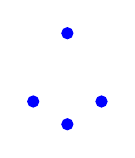
\begin{tikzpicture}\begin{axis}[axis equal, hide axis,
			ticks=none,
			enlargelimits=0,
			width=0.4*\hsize,
			axis lines=center,
			view={10}{20},
			ymin=1,ymax=7,
			xmin=0,xmax=6]

			\addplot [mark=*,color=blue] coordinates {(3,6)};
			\addplot [mark=*,color=blue] coordinates {(2,4)};
			\addplot [mark=*,color=blue] coordinates {(4,4)};
			\addplot [mark=*,color=blue] coordinates {(3,3.3333333)};
		\end{axis}\end{tikzpicture}
		&
		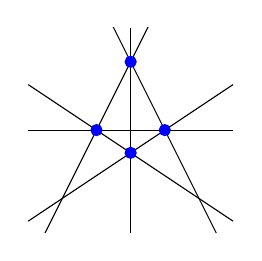
\begin{tikzpicture}\begin{axis}[axis equal, hide axis,
			ticks=none,
			enlargelimits=0,
			width=0.4*\hsize,
			axis lines=center,
			view={10}{20},
			ymin=1,ymax=7,
			xmin=0,xmax=6]

			\addplot [mark=*,color=blue] coordinates {(3,6)};
			\addplot [mark=*,color=blue] coordinates {(2,4)};
			\addplot [mark=*,color=blue] coordinates {(4,4)};
			\addplot [mark=*,color=blue] coordinates {(3,3.3333333)};

			\addplot [domain=0:6] {4};
			\addplot [domain=0:6] {-2*x+12};
			\addplot [domain=0:6] {2*x};
			\addplot [domain=0:6] {0.666666*x+1.3333333};
			\addplot [domain=0:6] {-0.66666*x+5.3333333};
			\addplot [mark=none] coordinates {(3, 1) (3, 7)};
		\end{axis}\end{tikzpicture}
		&
		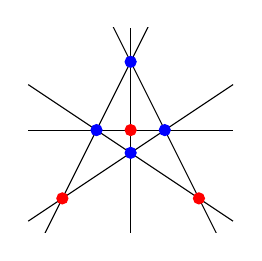
\begin{tikzpicture}\begin{axis}[axis equal, hide axis,
			ticks=none,
			enlargelimits=0,
			width=0.4*\hsize,
			axis lines=center,
			view={10}{20},
			ymin=1,ymax=7,
			xmin=0,xmax=6]

			\addplot [mark=*,color=blue] coordinates {(3,6)};
			\addplot [mark=*,color=blue] coordinates {(2,4)};
			\addplot [mark=*,color=blue] coordinates {(4,4)};
			\addplot [mark=*,color=blue] coordinates {(3,3.3333333)};

			\addplot [domain=0:6] {4};
			\addplot [domain=0:6] {-2*x+12};
			\addplot [domain=0:6] {2*x};
			\addplot [domain=0:6] {0.666666*x+1.3333333};
			\addplot [domain=0:6] {-0.66666*x+5.3333333};
			\addplot [mark=none] coordinates {(3, 1) (3, 7)};

			\addplot [mark=*,color=red] coordinates {(3,4)};
			\addplot [mark=*,color=red] coordinates {(1,2)};
			\addplot [mark=*,color=red] coordinates {(5,2)};
		\end{axis}\end{tikzpicture}
		\\
		$(S_0,L_0)$
		&
		$(S_1,L_1)$
		&
		$(S_2,L_2)$
	\end{tabular}\end{center}
	Ahora, veremos que $(S_n,L_n)$ no es un plano proyectivo axiomático, para
	ningún $n$. Para demostrarlo, procedemos por inducción.
	\begin{itemize}
		\item Trivialmente, $(S_0,L_0)$ no es un plano proyectivo axiomático,
			ya que cualesquiera dos puntos no están unidos por ninguna
			recta, (contradicción con \myref{1}).
		\item Suponemos, que $(S_{n-1},L_{n-1})$ no es un plano proyectivo
			axiomático y separamos en dos casos
			\begin{itemize}
				\item $n$ impar.
					\begin{itemize}
						\item Si no hemos añadido ninguna recta
							(en el paso de
							$(S_{n-1},L_{n-1})$ a
							$(S_nl_n)$), entonces
							$(S_n,L_n) = (S_{n-1},L_{n-1})$
							no es un plano proyectivo
							axiomático (por hipótesis).
						\item Si hemos añadido al menos una
							recta, por construcción esta
							(o estas) recta tiene
							únicamente dos puntos, por lo
							tanto, $(S_n,L_n)$ no cumple
							\myref{4}. Y $(S_n,L_n)$ no es
							un plano proyectivo axiomático.
					\end{itemize}
				\item $n$ par. 
					\begin{itemize}
						\item Si no hemos añadido nungún punto
							(en el paso de
							$(S_{n-1},L_{n-1})$ a
							$(S_n,L_n)$), entonces
							$(S_n,L_n) = (S_{n-1},L_{n-1})$
							no es un plano proyectivo
							axiomático (por hipótesis).
						\item Si hemos añadido al menos un
							punto, por construcción, este
							(o estos) punto, está contenido
							en dos únicas rectas. Pero, por
							el \hyperref[ej:2]{Ejercicio 2}
							sabemos que, en un plano
							proyectivo axiomático, el
							número de rectas que pasan por
							un punto y el número de puntos
							que contiene una recta son
							iguales. Con lo cual, si
							$(S_n,L_n)$ es un plano
							proyectivo axiomático y hay un
							punto por el que solo pasan
							dos rectas $\implies$ las
							rectas tienen 2 puntos,
							contradicción con \myref{4}.
							Y $(S_n,L_n)$ no es un plano
							proyectivo axiomático.
					\end{itemize}
			\end{itemize}
	\end{itemize}

	Por último, demostraremos que $(S,L)$ es un plano proyectivo axiomático. Para
	ello, veremos que cumple los axiomas uno a uno.
	\begin{enumerate}[\bf {A}1)]
		\item \textit{Para toda pareja de puntos $p,q \in S$, existe una única
			recta $l \in L$ tal que $p, q \in l$.} \\ \\
			Vemos de forma inmediata, que dados $p,q$ existe al menos una
			recta que los une, ya que, Si $p,q \in S_n$ y $p,q \notin
			S_{n-1}$, entonces, añadimos una recta que une $p$ y $q$ en
			$L_{n+1}$. La recta que une $p$ y $q$ es única ya que, antes de
			añadir una recta, comprobamos evitar duplicados.
		\item \textit{Para toda pareja de rectas $l_1, l_2$, $l_1 \cap l_2$
			es un punto de S.} \\ \\
			La intersección de dos rectas es como mínimo un punto, ya que
			si $l,r$ son rectas y $l,r \in L_n$ y $l,r \notin L_{n-1}$,
			entonces en $S_{n+1}$ añadimos un punto correspondiente a la
			intersección de $l$ y de $r$. Y la intersección es solo un
			punto ya que solo añadimos puntos por las rectas que no se
			intersequen ya.
		\item \textit{Existen puntos $p,q,r,s$ tal que todo subconjunto de 3
			elementos no se encuentran sobre la misma recta.} \\ \\
			Los cuatro puntos iniciales de $S_0$ cumplen este requisito.
			Puesto que a partir de $(S_2,L_2)$, no añadimos ninguna recta
			que pase por dos de ellos a la vez y en $(S_2,L_2)$, no están
			alineados.
		\item \textit{Cada recta contiene al menos 3 puntos.} \\ \\
			Si tenemos una recta $l$ tal que $l\in L_{2n+1}$, contiene, por
			construcción, al menos 2 puntos. Como en $L_{2n+2}$ hemos
			añadido al menos dos puntos, en $L_{2n+3}$ añadiremos al
			menos una recta $r$, por lo tanto, en $L_{2n+4}$ añadiremos al
			menos un punto (la intersección de $l$ y $r$) a $l$.
			Pasando $l$ a tener al menos 3 puntos.
	\end{enumerate}
\end{proof}

\begin{defi}[configuración desarguineana]
	Una configuración desarguineana es una pareja de puntos $D$ y un conjunto de
	rectas $R$ (dentro de un plano proyectivo), tal que cada punto de $D$ está
	contenido en, como mínimo 3 rectas de $R$, y cada recta de $R$, contiene al
	menos 3 puntos de $D$. Lo denotaremos como $(D,R)_\D$.
\end{defi}

\begin{ej}\label{ej:4}
	Comprobad que el teorema de Desargues da lugar a una configuración
	desarguineana con 10 puntos y 10 rectas.
\end{ej}
\begin{proof}
	Primero, recordemos el teorema de Desarges:

	Sean $ABC$, $A'B'C'$ dos triángulos en $\Po^2$ (sin vértices ni lados en común). Entonces,
	\[
		AA' \cap BB' \cap CC' \neq \emptyset \iff
		\begin{cases}
			AB \cap A'B' = Z \\
			AC \cap A'C' = Y \\
			BC \cap B'C' = X
		\end{cases}
		\text{ están alineados.}
	\]

	\begin{center}
		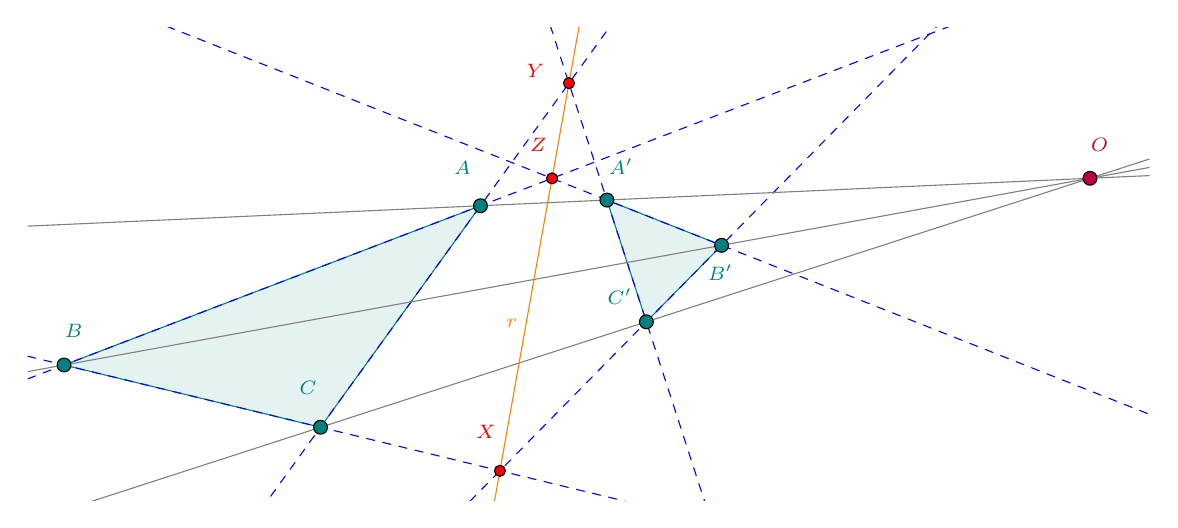
\begin{tikzpicture}[line cap=round,line join=round,>=triangle 45,x=1.5cm,y=1.5cm]
			\clip(-0.5,-0.5) rectangle (9.,3.5);
			\fill[line width=\pgflinewidth,color=teal,fill=teal,fill opacity=0.10000000149011612] (3.3336552362849274,1.992339795349051) -- (1.9793647349081451,0.1168150700088304) -- (-0.19217003454083312,0.6438220176250907) -- cycle;
			\fill[line width=\pgflinewidth,color=teal,fill=teal,fill opacity=0.10000000149011612] (4.403859447556563,2.040558909290155) -- (4.738313888759495,1.0095694436469795) -- (5.374944253774689,1.657128809689663) -- cycle;
			\draw [line width=\pgflinewidth,color=teal] (3.3336552362849274,1.992339795349051)-- (1.9793647349081451,0.1168150700088304);
			\draw [line width=\pgflinewidth,color=teal] (1.9793647349081451,0.1168150700088304)-- (-0.19217003454083312,0.6438220176250907);
			\draw [line width=\pgflinewidth,color=teal] (-0.19217003454083312,0.6438220176250907)-- (3.3336552362849274,1.992339795349051);
			\draw [line width=\pgflinewidth,color=teal] (4.403859447556563,2.040558909290155)-- (4.738313888759495,1.0095694436469795);
			\draw [line width=\pgflinewidth,color=teal] (4.738313888759495,1.0095694436469795)-- (5.374944253774689,1.657128809689663);
			\draw [line width=\pgflinewidth,color=teal] (5.374944253774689,1.657128809689663)-- (4.403859447556563,2.040558909290155);
			\draw [line width=\pgflinewidth,dashed=on 3.pt off 3.pt,color=blue,domain=-0.5:9.] plot(\x,{(--3.6701280196078825-0.383430099600492*\x)/0.9710848062181263});
			\draw [line width=\pgflinewidth,dashed=on 3.pt off 3.pt,color=blue,domain=-0.5:9.] plot(\x,{(--3.5541459610560944-1.8755247253402205*\x)/-1.3542905013767823});
			\draw [line width=\pgflinewidth,dashed=on 3.pt off 3.pt,color=blue,domain=-0.5:9.] plot(\x,{(--5.2228066883522954-1.0309894656431755*\x)/0.334454441202932});
			\draw [line width=\pgflinewidth,dashed=on 3.pt off 3.pt,color=blue,domain=-0.5:9.] plot(\x,{(--2.529148647580714--1.34851777772396*\x)/3.5258252708257607});
			\draw [line width=\pgflinewidth,dashed=on 3.pt off 3.pt,color=blue,domain=-0.5:9.] plot(\x,{(-1.2968069532830016--0.5270069476162603*\x)/-2.171534769448978});
			\draw [line width=\pgflinewidth,dashed=on 3.pt off 3.pt,color=blue,domain=-0.5:9.] plot(\x,{(-2.425616974499177--0.6475593660426835*\x)/0.6366303650151943});
			\draw [line width=\pgflinewidth,color=gray,domain=-0.5:9.] plot(\x,{(--9.50601349361014--0.23250306512482055*\x)/5.1603138069701515});
			\draw [line width=\pgflinewidth,color=gray,domain=-0.5:9.] plot(\x,{(--1.9667522247370517-1.215273416826892*\x)/-3.7556551544955843});
			\draw [line width=\pgflinewidth,color=gray,domain=-0.5:9.] plot(\x,{(--2.1171944617344565--0.5677140507842084*\x)/3.11902478948039});
			\draw [line width=\pgflinewidth,color=orange,domain=-0.5:9.] plot(\x,{(--2.855613634592153-0.8059659723881762*\x)/-0.14358796715525868});
			\begin{scriptsize}
				\draw [fill=purple] (8.49396904325508,2.2248428604738715) circle (2.5pt);
				\draw[color=purple] (8.5756934700623,2.511596640794484) node {$O$};
				\draw [fill=teal] (3.3336552362849274,1.992339795349051) circle (2.5pt);
				\draw[color=teal] (3.1818813007858053,2.3100939843529726) node {$A$};
				\draw [fill=teal] (-0.19217003454083312,0.6438220176250907) circle (2.5pt);
				\draw[color=teal] (-0.1104456077336135,0.9305757979457029) node {$B$};
				\draw [fill=teal] (1.9793647349081451,0.1168150700088304) circle (2.5pt);
				\draw[color=teal] (1.8742904718702913,0.4500694633544068) node {$C$};
				\draw [fill=teal] (4.403859447556563,2.040558909290155) circle (2.5pt);
				\draw[color=teal] (4.52449688404727,2.3255941886946276) node {$A'$};
				\draw [fill=teal] (4.738313888759495,1.0095694436469795) circle (2.5pt);
				\draw[color=teal] (4.512821965931953,1.2250796804371424) node {$C'$};
				\draw [fill=teal] (5.374944253774689,1.657128809689663) circle (2.5pt);
				\draw[color=teal] (5.365090988350101,1.4265823368786539) node {$B'$};
				\draw [fill=red] (4.082899471593713,3.029950328105273) circle (2.0pt);
				\draw[color=red] (3.8006519608976106,3.1316048144606725) node {$Y$};
				\draw [fill=red] (3.939311504438454,2.223984355717097) circle (2.0pt);
				\draw[color=red] (3.8240017971282447,2.511596640794484) node {$Z$};
				\draw [fill=red] (3.498235188833963,-0.2517976241139916) circle (2.0pt);
				\draw[color=red] (3.3803549087461957,0.07806455915469361) node {$X$};
				\draw[color=orange] (3.6,1) node {$r$};
			\end{scriptsize}
		\end{tikzpicture}
	\end{center}
	\noindent Evidentemente, como se puede observar, en la imagen hay una
	configuración desarguineana de 10 puntos y 10 rectas.
	\[
		\begin{cases}
			\text{Por $A$ pasan $\overline{AC}$, $\overline{AB}$ y
			$\overline{AA^\prime}$.} \\
			\text{Por $B$ pasan $\overline{BA}$, $\overline{BC}$ y
			$\overline{BB^\prime}$.} \\
			\text{Por $C$ pasan $\overline{CA}$, $\overline{CB}$ y
			$\overline{CC^\prime}$.} \\
			\text{Por $A^\prime$ pasan $\overline{A^\prime B^\prime}$,
			$\overline{A^\prime C^\prime}$ y $\overline{A^\prime A}$.} \\
			\text{Por $B^\prime$ pasan $\overline{B^\prime A^\prime}$,
			$\overline{B^\prime C^\prime}$ y $\overline{B^\prime B}$.} \\
			\text{Por $C^\prime$ pasan $\overline{C^\prime A^\prime}$,
			$\overline{C^\prime B^\prime}$ y $\overline{C^\prime C}$.} \\
			\text{Por $O$ pasan $\overline{AA^\prime}$,
			$\overline{BB^\prime}$ y $\overline{CC^\prime}$.} \\
			\text{Por $X$ pasan $\overline{BC}$,
			$\overline{B^\prime C^\prime}$ y $\overline{XYZ}$.} \\
			\text{Por $Y$ pasan $\overline{AC}$,
			$\overline{A^\prime C^\prime}$ y $\overline{XYZ}$.} \\
			\text{Por $Z$ pasan $\overline{AB}$,
			$\overline{A^\prime B^\prime}$ y $\overline{XYZ}$.}
		\end{cases}
		\quad
		\begin{cases}
			\text{$\overline{AA^\prime}$ contiene a $A$, $A^\prime$ y
			$O$.} \\
			\text{$\overline{BB^\prime}$ contiene a $B$, $B^\prime$ y
			$O$.} \\
			\text{$\overline{CC^\prime}$ contiene a $C$, $C^\prime$ y
			$O$.} \\
			\text{$\overline{AB}$ contiene a $A$, $B$ y $Z$.} \\
			\text{$\overline{AC}$ contiene a $A$, $C$ y $Y$.} \\
			\text{$\overline{BC}$ contiene a $B$, $C$ y $X$.} \\
			\text{$\overline{A^\prime B^\prime}$ contiene a $A^\prime$,
			$B^\prime$ y $Z$.} \\
			\text{$\overline{A^\prime C^\prime}$ contiene a $A^\prime$,
			$C^\prime$ y $Y$.} \\
			\text{$\overline{B^\prime C^\prime}$ contiene a $B^\prime$,
			$C^\prime$ y $X$.} \\
			\text{$\overline{XYZ}$ contiene a $X$, $Y$ y $Z$.}
		\end{cases}
	\]
\end{proof}

\noindent Lo que finalmente veremeos es que el plano proyectivo libre $(S,L)$ no
contiene configuraciones desarguineanas, y por tanto en \'el no se puede dar el teorema
de Desargues.

\begin{ej}\label{ej:5}
	Demostrad que si una configuración desarguineana finita $(D,R)_\D$ está
	contenida en $(S,L)$, entonces estaba contenida en $(S_0,L_0)$. Concluid
	que en $(S,L)$ el teorema de Desargues no es cierto. (\emph{Indicación:}
	para cada $p \in D$, el nivel de $p$ es el valor de $n$ para el cual
	$p \in S_n$ y $p \notin S_{n-1}$. Definiendo similarmente el nivel de una recta
	en $R$. Estudiar cómo se origina el punto, o la recta, con nivel más grande
	de $(D,R)_\D$).
\end{ej}
\begin{proof}
	Suponemos que existe $(D,R)_\D$ una configuración desarguineana finita en
	$(S,L)$. Consideramos ahora, $p \in D$ uno de los puntos con nivel más alto de
	la configuración (tomando la definición de nivel dada en el enunciado). Si $p$
	se añade a $S_n$ (donde $n$ es el nivel de $p$) como intersección de dos
	rectas, como la configuración es desarguineana y $p$ es el punto de nivel más
	alto, se añade una recta $l \in R$ a $L_{n+1}$ que pasa por $p$ (y
	$l \notin L_n$). Pero, por construcción esta recta solo tiene 2 puntos, luego
	en un paso posterior se añade un punto $q \in D$ a $l$ ($l$ tiene al menos tres
	puntos, por ser parte de una configuración desarguineana). Lo cual es una
	contradicción con que $p$ es uno de los puntos con nivel más alto de
	$(D,R)_\D$. Es decir, o bien $(D,R)_\D$ no existe, o $p$ no se añade como 
	intersección de dos rectas.
	
	Si $p$ no se añade como intersección de dos rectas, necesariamente estaba en
	$S_0$, y por ser de nivel más alto, $D \subseteq S_0$. Pero si todos los puntos
	de $(D,R)_\D$ estan en $S_0$, todas las rectas están en $L_0$, ya que si
	$l \in L_n$ y $l \notin L_{n-1}$, por construcción $l$ solo contiene 2 puntos
	de $S_{n-1}$.
	\\ \\
	\noindent Como $(S_0,L_0)$, no contiene ninguna configuración desarguineana
	finita, no existe ninguna configuración desarguineana finita en $(S,L)$. Por
	lo tanto, el teorema de Desargues es falso en $(S,L)$ (el teorema de desargues
	garantiza una configuración desarguineana finita por el
	\hyperref[ej:4]{Ejercicio 4}).
\end{proof}
\end{document}
